\chapter{Analysis of the Neural Engineering Framework}
\label{chapt:analysis}

In this chapter, we provide a thorough examination of the Neural Engineering Framework~\citep[NEF;][]{eliasmith2003a} that is not currently published elsewhere.
The goals are two-fold: (1)~explore the consequences of its computational principles at a theoretical level, and in doing so debunk some of the common myths that have become associated with the NEF since its inception, and (2)~assess its suitability as a framework for deploying SNNs on neuromorphic hardware by analyzing its scalability, correctness, efficiency, Turing-completeness, robustness, and extensibility.\footnote{
To help delineate separate considerations, some sub-sections may be significantly shorter than others.
}
% This involves a proof of equation~\ref{eq:rate-approximation} thatextends and improves the discussion of \citet[][pp.~132--136]{eliasmith2003a} to provide a sufficient criteria for the correctness of the first two principles of the NEF at the level of individual spikes.
% The correctness of the third principle is proven in \citet[][pp.~221--225]{eliasmith2003a} and is extended by various proofs in section~\ref{sec:synaptic-extensions}.

\section{Computational Sub-Principles}

In this section, we focus primarily on the third principle of the NEF, and elucidate some high-level observations, or ``sub-principles'', that follow from its adoption.
In particular, \TODO{...}

\subsection{Single-layer equivalence}

In section~\ref{sec:nef}, we focused primarily on a single recurrently connected population of neurons.
However, any multi-layer NEF network, where each layer may be recurrent, and feedforward connections and feedback connections may also be included between distant layers -- may be rewritten as a single recurrently connected population.
Indeed, even for models as complex as Spaun~\citep{eliasmith2012, choo2018}, the Nengo builder strips away the model specification, and leaves only channels that transmit spikes, and transfer functions that operate on these spikes~\citep{bekolay2014, gosmann2017automatic}.
The topology of the network encodes spatial and organizational structure (e.g.,~hierarchies), which may be used to constrain and inform the design of biological models, and to aid in understanding function.
The mechanisms underneath are mere signals and operators, all coupled to one another to compute some dynamical system.

To examine some of the consequences of this observation, we assume without loss of generality that there are $m$ layers, and each of the layers uses $n$ neurons to represent a $q$-dimensional state-vector.
The procedure for rewriting the network is as follows:
\begin{enumerate}
\item Stack all of the populations together into a single layer that consists of $nm$ neurons. 
\item Stack all of the state-vectors together into one vector, $\V{x}(t) \in \mathbb{R}^{qm}$, to represent the global state-space.
\item Construct the encoding matrix, $E \in \mathbb{R}^{nm \times qm}$, by inserting the $i^\text{th}$ encoding matrix into the $(i\text{,} i)^\text{th}$ block, such that $E$ is in block-diagonal form (note: there are $m \times m$ blocks and each is $n \times q$).
\item Construct the decoding matrix, $D^\V{f} \in \mathbb{R}^{nm \times qm}$, by inserting each decoding matrix $D^{\V{f}_{i\text{,}j}}$ into the $(i\text{,} j)^\text{th}$ block, where $\V{f}_{i\text{,}j}$ is the function computed between the $i^\text{th}$ presynaptic population and the $j^\text{th}$ postsynaptic population.
\end{enumerate}
Then Principles~1--3 apply in the same way to this single population, while being functionally equivalent to the original network.

This reveals that the problem of constructing and training arbitrary network topologies may be reduced to the special case of a single layer.
Conversely, we do not lose any computational power by limiting our focus to a single layer.
However, the encoding matrix is extremely sparse with $(m - 1) / m$ percent of its coefficients set to zero.
Likewise, the block-structure of the decoding matrix is isomorphic to the graph structure of the original network.

This characterizes the functional role of network structure as: partitioning the global state-space into a union of state-vectors, sparsifying its encoders, and arranging the decoders into a block-structure that mirrors the interactions between sub-spaces.
In terms of computation, this structure dramatically reduces the time and memory requirements that would otherwise be needed for a full-rank $nm \times nm$ matrix multiplication.
In terms of training, the challenges involved in globally optimizing an RNN may be viewed under the lens of identifying relatively low-dimensional sub-spaces and their interactions with one another.

\subsection{Heterogeneous dynamical primitives}

An important observation is that neurons~(equation~\ref{eq:lif-model}), synapses~(equation~\ref{eq:lowpass-impulse}), and even the functional behaviour of entire recurrent networks~(equations~\ref{eq:discrete-dynamical-system} and~\ref{eq:lti}), can all be described in terms of differential equations.
These ``dynamical primitives'' all have certain filtering properties, linear and nonlinear transfer functions, and internal states that evolve over time in response to some input in order to produce some output.

On the other hand, a central insight from deep learning is that a variety\footnote{
The variety of nonlinear responses comes from the distribution of weights and biases, analagous to the hetereogeneity obtained in equation~\ref{eq:encoding} via encoding vectors, gains, and biases.}
of static nonlinear functions, when structurally composed, enhances the \emph{spatial complexity} of network function.
An analagous insight in the above context is that a variety of transfer functions, when temporally composed, enhances the \emph{dynamical complexity} of network function.
In particular, the time-constants of synapses, neuron leakages, and recurrent network dynamics -- all act along different time-scales.
In effect, NEF networks compose rich temporal functions by leveraging dynamical primitives that are heterogeneous in time.
A compelling example is provided in section~\ref{sec:delay-lstm} that applies BPTT to a deep recurrent NEF network to predict a chaotic time-series.

\subsection{Duality of macroscopic and microscopic dynamics}

As a corollary to the previous observation,
once all primitive operations are expressed in the same language (i.e.,~differential equations), they become both \emph{composable} and \emph{interchangeable}.
To the point of interchangeability, one can implement a lowpass filter by using a single synapse, or by training a population to emulate the same dynamical system via Principle~3.
To the point of composability, one can substitute the transfer function of a single synapse with that of an entire recurrent network.

We illustrate this with a specific example by considering the following architecture:
$$A \rightarrow (B \rightarrow B) \rightarrow A \text{,}$$
where $A$ and $B$ are separate neural ensembles and ``$\rightarrow$'' denotes a synaptic weight matrix.
That is, $B$ is locally-recurrent, and $A$ is globally-recurrent via the outer loop through $B$.
We may encapsulate $H := B \rightarrow B$ as a dynamical primitive, and then \emph{re-interpret} the whole system as:
$$A \rightarrow_H A \text{,}$$
where ``$\rightarrow_H$'' denotes some weight matrix where the synapse model has been replaced by $H$ --
akin to a ``virtual'' synapse, whose dynamics are implemented by $B$ under the hood.
This is simply a mathematical ``trick''.
But the practical point is that we can use the same theory and the same tools to understand the composition and substitution of these systems.
This is made possible since we employ a common language and framework for describing and leveraging dynamical systems.

In section~\ref{sec:linear-extensions}, this idea forms the basis of our proofs that extend Principle~3.
In section~\ref{sec:pure_delay}, we demonstrate a method of systematically harnessing miniature delays in axonal spike-transmission to improve the accuracy of longer network-level delays.

\TODO{example application in section~\ref{sec:applications} -- if $B \rightarrow B$ is a delay network, we can then use what we know about amplifying axonal spike delays to make an even longer delay out of the entire system}

\subsection{Unpredictability, chaos, and strange attractors}

An apparent misconception associated with NEF networks is that we already ``understand'' the computations being engineered into the network, and therefore have nothing to learn from such simulations.
But just because a network's function can be written down using equations, does not mean that its effects are fully understood ahead of time.
For example, the NEF has been used to construct chaotic systems, such as the Lorenz strange attractor~\citep{eliasmith2005b}.
This \emph{deterministic} system is fully described by a three-dimensional nonlinear dynamical system.
However, due to the nature of such chaotic systems, arbitrarily small perturbations in state-space diverge exponentially quickly over time up to the diameter of the attractor~\citep[][pp.~328--330]{strogatz2000nonlinear}.
This leads to a fundamental inability to predict the trajectory of any physical instantiation of the system; the time-horizon that can be predicted, within some given tolerance, scales only logarithmically with the precision of the observer.

More to the point, this accusation is theoretically equivalent to suggesting the same of any algorithm or computer program for that matter.
Even though \emph{any} computer program can be written down using a finite set of symbolic expressions, and realized as a discrete sequence of steps that dynamically evolve a set of registers---such as the machine of \citet{turing1938computable}---does not mean that we know what that program will compute ahead of time on any given input.
The assertion that the behaviour of certain programs are in essence ``unpredictable'' corresponds to the notion of \emph{undecidability} in formal theories of computation; informally, most non-trivial programs need to be run in order to see what they will do with their inputs.

This discussion extends to dynamical systems, where chaos and undecidability are also interwoven~\citep{moore1991generalized}.
For example, suppose we take the linear time-invariant~(LTI) system of equation~\ref{eq:lti} and then include saturation within each of the state-variables (such that their absolute magnitudes cannot exceed one).
Surprisingly, this is a sufficient route to chaos.
The inclusion of this single nonlinearity spawns attractors with properties that are undecidable~\citep{blondel2001stability}; basic questions about the system's response cannot be resolved in a finite number of steps.
This example is of special interest to us since the LIF neuron (equation~\ref{eq:lif-model}) exhibits a similar saturation effect, namely $r(\V{v}) \le \tau_\text{ref}^{-1}$, where the upper-bound is approached as $\V{x}(t) \in \mathbb{R}^q$ extends beyond the representational range established by the encoding parameters selected by Principle~1.
It follows that even the most basic spiking instantiation of Principle~3 must, in general, be simulated in order to determine its behaviour whenever the input signal drives the state-space outside the range of neural representation.
Notably, this saturation effect is exploited to overload working memory with sequential items in the Spaun model~\citep{eliasmith2012}, which suggests that the model behaviour is chaotic at multiple levels of analysis.

\begin{figure}
    \centering
    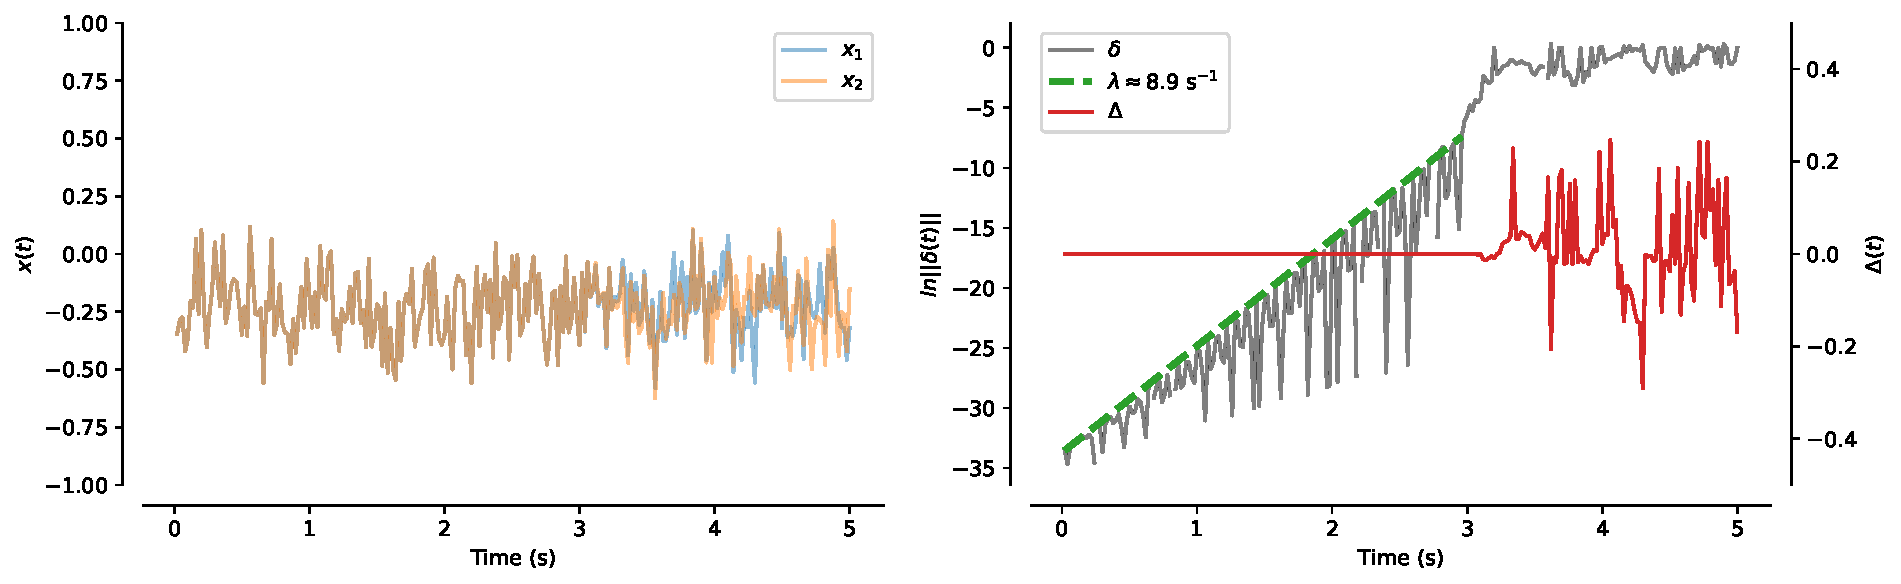
\includegraphics[width=\textwidth]{chaotic-integrator}
     
    \caption{\label{fig:chaotic-integrator} 
      An autonomous scalar integrator---the simplest possible recurrent SNN, built using the NEF---exhibiting chaotic neural dynamics.
      (Left)~Two deterministic simulations of the exact same network.
          One is initialized to $x_1(0) = 0$, and the other to $x_2(0) = \numprint{e-15}$.
          Both simulations fall into the same strange attractor, close to zero.
      (Right)~Plotting the difference in representational states~($\Delta$) and neural states~($\delta$) on a logarithmic scale.
          The neural states diverge exponentially quickly---leaping 30 orders of magnitude in 3 seconds---according to $\| \delta(t) \| \approx \bigoh{e^{\lambda t}}$.
          The representational difference is essentially zero until $\delta$ hits the diameter of the attractor.
          It is physically impossible to predict the future state of this system beyond a time-scale of $\bigoh{\lambda^{-1}} \approx 0.1$~seconds (see text for details).
    }
\end{figure}

Perhaps even more surprisingly, one does not need to invoke any saturation to observe chaos, at the level of individual neurons, in NEF networks implementing linear dynamics.
For example, consider the one-dimensional, autonomous (i.e.,~no input), integrator:
$$\dot{x}(t) = 0 \text{,}$$
implemented as an SNN using Principle~3 of the NEF ($A = B = D = 0$, $C = 1$).
This is perhaps the simplest recurrent network that one can imagine; a line attractor without input, that is to hold its initial state indefinitely.
Nevertheless, as shown in Figure~\ref{fig:chaotic-integrator}, the neural states display the tell-tale signs of a strange attractor~\citep[cf.~][Figure~9.3.5]{strogatz2000nonlinear}.
Specifically, let $\V{v}_1(t), \V{v}_2(t) \in \mathbb{R}^n$ be two voltage vectors (see equation~\ref{eq:lif-model}) from two separate, but deterministic simulations, of the \emph{exact} same network ($n = 10$, $\tau = 5$\,ms, $\dt{} = 0.1$\,ms, down-sampled every $20$\,ms).
The first simulation is initialized to the default of $x_1(0) = 0$, while the second is initialized to $x_2(0) = \numprint{e-15}$.
% Both fall into the same attractor basins, decoding an approximation of $0$, that persists indefinitely through recurrent feedback.
Now let:
\begin{align*}
\Delta(t) &= x_1(t) - x_2(t) \\
\delta(t) &= \V{v}_1(t) - \V{v}_2(t) \text{,}
\end{align*}
be the difference in representational state and neural state, respectively.
We find that $\Delta$ remains bounded above by the accuracy of neural representation, as expected.
However, $\delta$ diverges exponentially over time, indicating that the neural states are within a strange attractor (the Lyapunov exponent $\lambda \approx 8.9$\,s${}^{-1}$ gives the exponential rate of divergence); the voltage vectors are tracing out a fractal manifold embedded within an $n$-dimensional space that cannot be predicted beyond a time-horizon on the order of $\bigoh{\lambda^{-1}} \approx 0.1$\,s.
Despite this, the NEF is capable of taming the chaos at the neural level and providing a robust estimate at the population level, due to the correspondance between each strange attractor and a stable point in representational space~\citep[][p.~237]{eliasmith2003a}.

More generally, the NEF may be used to implement arbitrary algorithms encoded as dynamical systems (see section~\ref{sec:nef-turing}), which implies that it is not exempt from computational-complexity theory. 
Networks can perform interesting tasks via algorithmic manipulations of inputs and states~\citep{choo2018}.
And, in this case, the network must in general be explicitly simulated in order to carry out the computations of said algorithm.
At the same time, the NEF provides a framework for understanding the dynamical transformations being performed, examining relationships between structure and function, relating these functions to neurobiological systems, and compiling them onto neuromorphic hardware.

\TODO{Forward reference where this disputes deneve's methods}

\iffalse
\subsection{Continuous-Time and Discrete-Time}

The idea that both continuous-time and discrete-time dynamics play important roles at different time-scales, both in terms of the dominant dynamics and in terms of the desired computation.
It is also important to consider both for neuromorphic hardware.
\fi

\subsection{Postsynaptic current coding}
\label{sec:psc-coding}

A long-standing debate in neuroscience has traditionally revolved around the question of whether biological neurons transmit information using a ``rate code'' in which the information is encoded by the firing rates of individual neurons~\citep{adrian1928basis}, or a ``spike-timing code'' in which information is encoded by the precise temporal patterns of spike trains~\citep{rieke1999spikes} or likewise their temporal order in relation to one another~\citep{thorpe1998rank}.
However, there is historically little consensus between neuroscientists as to what exactly consistutes a rate code~\citep[][pp.~89--91]{eliasmith2003a}.

\citet{gerstner1999spiking} observes that there are at least three different ways to define a rate code, and that in many important ways they are consistent with that of a timing-based code.
\citet{fairhall2001efficiency} examines the adaptive dynamics of neurons in a fly's visual system and concludes that the principles of its code depend on the time-scales of interest.
\citet{brette2015philosophy} argues that the question about which code the brain uses is irrelevant, and should be replaced by one that instead addresses the causal role of neural activity.
\citet{eliasmith2003a} likewise proposes that we should focus on the physical instantiation, and functional consequences therein, of any given approach to neural coding, rather than resorting to semantic labels that are ultimately irrelevant. 

\begin{figure}
    \centering
    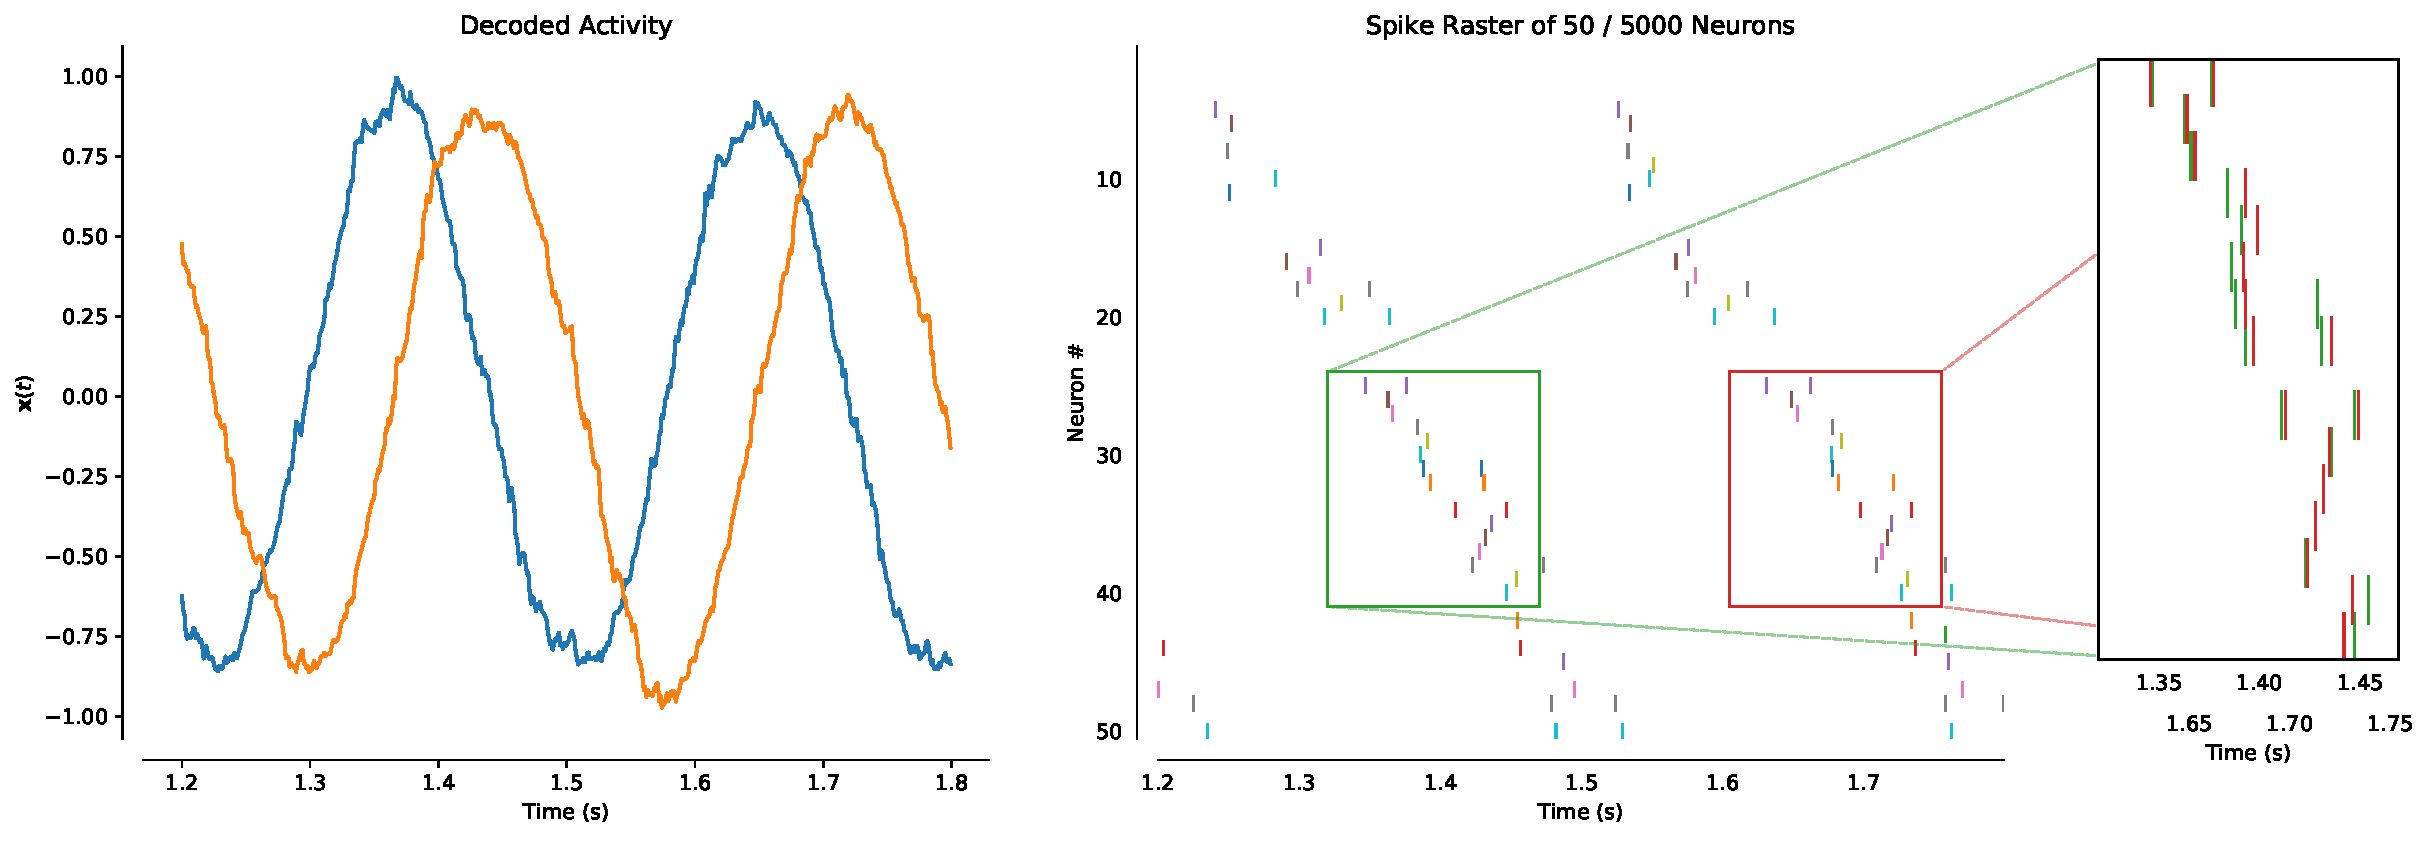
\includegraphics[width=\textwidth]{spike-time-coding}
     
    \caption{\label{fig:spike-time-coding} 
      Demonstrating the irrelevance of identifying a ``spike-time code'' versus a ``rate code'' in the context of a standard NEF-optimized network.
      We define this as a ``postsynaptic current code'' instead.
      (Left)~An ensemble of LIF neurons are trained to oscillate at approximately $3.5$\,Hz.
      (Right)~Spike rasters of \numprint{50} randomly selected neurons, ordered by their encoding vector's polar angle.
      Each neuron spikes only $0$, $1$, or $2$ times per oscillation, and at a precise moment in time---on the order of milliseconds (see inset)---before remaining silent for another couple hundred milliseconds.
      Thus, the precise spike-timing of each individual neuron reliably conveys information about the state-space of the oscillation, despite never explicitly incorporating such a requirement about timing into the training procedure.
    }
\end{figure}

Nevertheless, many have mislabelled the NEF as employing a rate-coding scheme [personal communication], including \citet{lagorce2015stick} and~\citet{frady2019robust} for two recent examples -- we refer to these two below, to illustrate why this accusation constitutes a damaging use of semantics.
% On one hand, we understand that this is due to the way in which the optimization procedure is most often simplified using equation~\ref{eq:rate-approximation}.
Specifically, this micharacterization has lead to the misapplication of many criticisms~\citep{gautrais1998rate} that stem from the original proposal of \citet{adrian1928basis}, namely the need to average spike rates over long windows of time.
We find this important to clarify because it leads to imprudent conclusions or ``myths'' about the NEF such as those claimed in \citet{lagorce2015stick, frady2019robust}:
\begin{enumerate}
\item The NEF does not exhibit precise sequences of action-potentials.
\item The NEF does not support high speed neural computation.
\item The NEF does not display rhythmic activity.
\item The NEF requires very large numbers of neurons to compute simple functions.
\end{enumerate}
We now debunk each of these claims in turn.
For the first three, we refer to the same simulation depicted in Figure~\ref{fig:spike-time-coding}.
This simulation applies the NEF, as described in section~\ref{sec:nef}, to the case of an autonomous two-dimensional oscillator ($n = \numprint{5000}$, $\tau = 0.1$\,s, $\dt{} = 1$\,ms).
The encoding parameters are randomly tiled across the two-dimensional state-space such that each neuron only responds to 25\% of the state's projection onto its encoder (i.e.,~uniform $[0.5, 1)$ intercepts), and each neuron \emph{would} fire at a rate of $20$--$40$\,Hz if encoding a constant state with maximal similarity to its encoder.
As we explain, the firing statistics are not at all characterized by $20$--$40$\,Hz spike-trains.
We omit the first $1.2$ seconds of simulation to wash away initial transients.

\paragraph{1. The NEF can exhibit repeatedly precise sequences of action-potentials.}

See Figure~\ref{fig:spike-time-coding}~inset.
When comparing the spike-trains between two separate oscillations at the same phase, not only is the order of spiking consistent, as in rank order cording~\citep{thorpe1998rank}, but also the precise spike-timing ($\pm$ a couple milliseconds).

\paragraph{2. The NEF readily supports high speed neural information processing.}

In our example, neurons respond quickly to encode the rapidly-fluctuating oscillatory state, and do so without any system-level ``delay'' or undersired filtering.\footnote{
The postsynaptic filter that is applied is leveraged to participate in the required computation (see Principle~3; section~\ref{sec:principle3}).
There is no unwanted phase-shift.
}
As will be explained in section~\ref{sec:scalability}, the precision of a feed-forward network scales as $\bigoh{\tau \sqrt{n}}$.
Thus, one is free to set the synaptic time-constant arbitrarily small, so long as the number of neurons are increased in proportion.
We have verified this both theoretically and numerically.
This enables arbitrarily fast transmission of information throughout the network assuming the criteria of section~\ref{sec:spike-coding} is met (see also Figure~\ref{fig:poisson-frequency-scaling}).
Yet, even when constrained to longer time-constants, section~\ref{sec:deep-delay-networks} demonstrates a novel deep NEF network that is capable of \emph{instantaneously} propagating low-frequency stimuli through 8 layers of synaptic filters ($\tau = 0.1$\,s).

\paragraph{3. The NEF examples that invoke Principle~3 all display rhythmic activity.}

The NEF was designed as a toolkit for modelling dynamic rhythmic activity~\citep{eliasmith1999developing} such as the central pattern generator driving lamprey locomotion~\citep{eliasmith2000b}.
Indeed, Figure~\ref{fig:spike-time-coding} clearly displays rhythmic activity at both the population level~(see left) and activity level~(see right).
The properties of these rhythms can be understood as arising from the dynamics of the postsynaptic currents, in response to the neural encoding of the state-vector governed by some underlying set of differential equations.

\paragraph{4. The NEF can compute difficult functions with any number of neurons.}

See Figure~\ref{fig:chaotic-integrator} for an example of ten spiking LIF neurons implementing a line attractor ($\tau = 5$\,ms), or section~\ref{sec:delay-lstm} for a six neuron cell that outperforms LSTM cells.
No matter how complex the function, the mandate of the NEF is to leverage its neuron models as a basis for that function. 
Sometimes this can be done with sufficient accuracy using a single neuron, and in other cases one might need a few million or even more.
In general, the feed-forward precision scales as $\bigoh{\tau \sqrt{n}}$ while the dynamical precision scales as $\bigoh{\sqrt{n}}$ (under fairly weak assumptions; see section~\ref{sec:scalability}).
But one cannot consider the questions of resource usage and functional precision within a vacuum.
One must resolve such questions with respect to the device-level models of the physical hardware implementation as well as the intended target application.
Some advances in this direction are underway~\citep{schwemmer2015constructing, thalmeier2016learning}.
But many other considerations such as weight factorization, mechanistic constraints, and the energy consumed by different synaptic or neural operations, may all play a role.
If one is interested in constructing functioning dynamical SNNs using neuromorphic hardware, we suggest that one considers all such factors in the context of the target application before labelling an approach as being unequivocally inferior.

The confusion surrounding rate coding in the NEF has essentially risen from the adoption of equation~\ref{eq:rate-approximation}.
However, as we have said, this merely reformulates the optimization procedure to be more efficient, without sacrificing correctness as proven in section~\ref{sec:spike-coding}.
We remark that, in Figure~\ref{fig:spike-time-coding}, the firing statistics are completely unlike their rate-model counterparts, despite the target postsynaptic currents and overall system dynamics remaining the same.
That is, each neuron only fires at an average rate of $3$\,Hz across the simulation, much slower than the $20$--$40$\,Hz rate that they would fire at for constant inputs.
Likewise, the postsynaptic impulse response that results from a single spike, decays to a factor of $e^{-\frac{10}{3}} \approx 3.5\%$, before \emph{that same} neuron triggers another spike, on average.
of the synaptic filter.
In general neither the average rates, inter-spike intervals, nor spike times tell the entire story.

But then, how does equation~\ref{eq:rate-approximation} hold if each neuron is not spiking at its intended rate?
Our proposal to resolve this seemingly paradoxical situation is to first establish a new label: ``postsynaptic current code''.
This code does not care about the spike-rates of individual neurons; it is only sensitive to how well the weighted and synaptically-filtered spikes, \emph{when pooled across the entire population}, approximate some desired set of postsynaptic currents (corresponding to an affine transformation of the required state-vector)~\citep{tripp2006neural}.
This is summarized by taking the encoding equation~\ref{eq:encoding} and decoding equation~\ref{eq:trans-decode} which fold into the weight equation~\ref{eq:factored-weights} -- and combining them in a similar manner to \citet{stoeckel2018}:
\begin{equation} \label{eq:psc-code}
\alpha_i \left\langle \V{e}_i\text{,}\, \V{x}(t) \right\rangle + \beta_i \approx \sum_{j=1}^n \sum_m \omega_{ij} h \left( t - t_{j\text{,}m} \right) \text{.}
\end{equation}
In plain words, the represented state-vector is linearly projected onto the postsynaptic current of each neuron. 
How this works in light of equation~\ref{eq:rate-approximation} requires careful proof, and the subtleties surrounding why this can matter are often lost even amongst experts in the field~[personal communication].
But as our example illustrates, the NEF cannot be adhering to any single definition of rate or timing code.
Rather, it is representing desired transformations by mapping latent state-variables onto postsynaptic currents.  %, with precision that scales as $\bigoh{\tau \sqrt{n}}$.
% Anectodally, we find that it takes at least several months of working closely with the details of NEF simulations to appreciate these nuances, although the software package Nengo dramatically assists in abstracting them away from the user.
% Later, we participate in further attempts to rectify these misunderstandings using detailed proofs and simulation results in order to tease apart the NEF's coding principles, scaling properties, and sources of error.

If one is still unconvinced, then, as mentioned in section~\ref{sec:relationships} when comparing the NEF to RC and FORCE, one can forego the substitution of equation~\ref{eq:rate-approximation} and perform the optimization directly in the spiking time-domain~\citep{voelker2016a, duggins2017incorporating}, or even apply backpropagation through time~\citep{rasmussen2018nengodl}.
But the fact of the matter is that this becomes unnecessary (and inefficient) for a large class of interesting systems and models that we commonly explore.
% We further step outside this paradigm for conductance-based synapses, and adaptive LIF neurons.

% https://link.springer.com/content/pdf/10.1023/B:NACO.0000027755.02868.60.pdf


\subsection{Energy-minimization via low-frequency representation}

We define a \emph{low-frequency representation} as one in which the represented vector, $\V{x}(t)$, carries its information within frequencies on the order of the cut-off frequency of the synaptic filter.
That is, $\bigoh{\left( 2 \pi \tau \right)^{-1}}$\,Hz, where $\tau$ is the synaptic time-constant of equation~\ref{eq:lowpass-laplace} in seconds.\footnote{
For example, a typical time-constant of $\tau = 5$\,ms would imply that most information is present within a frequency band of $< 32$\,Hz.
}
Such representations are known to be ubiquitous in biological systems~\citep{pulvermuller1997high, singer1999neuronal, szendro2001bio}.
The NEF provides a basic theoretical explanation for this observation from the perspective of energy-minimization.

As discussed in the previous section, and described by equation~\ref{eq:psc-code}, the state-vector $\V{x}(t)$ is projected onto postsynaptic currents.
To analyze the frequency content of this code, we apply the Laplace transform to both sides of equation~\ref{eq:psc-code}, and substitute in the synapse model from equation~\ref{eq:lowpass-laplace}:
\begin{equation} \label{eq:psc-code-laplace}
\begin{aligned}
\alpha_i \left\langle \V{e}_i\text{,}\, \laplace{ \V{x}(t) }(s) \right\rangle + \beta_i &\approx \sum_{j=1}^n \sum_m \omega_{ij} \laplace{ h \left( t - t_{j\text{,}m} \right) }(s) \\
&= \sum_{j=1}^n \sum_m \omega_{ij} \frac{e^{-{t_{j\text{,}m}s}}}{\tau s + 1} \\ 
&= \left( \tau s + 1 \right)^{-1} \underbrace{ \sum_{j=1}^n \omega_{ij} \laplace{ a_j(t) }(s) }_{G_i(s)} \text{.}
\end{aligned}
\end{equation}
$G_i(s)$ is defined as the Laplace transform of the weighted combination of presynaptic (unfiltered) spike-trains.
The magnitude of $| G(2\pi i f) |$, evaluated at real frequencies $f$, is a (dimensionless) measure of the absolute power required to drive all of the synapses of the $i^\text{th}$ postsynaptic neuron, in order to generate such a PSC.
Rearranging equation~\ref{eq:psc-code-laplace} yields:
\begin{equation} \label{eq:psc-code-rearranged}
G_i(s) \approx \left( \tau s + 1 \right) \left( \alpha_i \left\langle \V{e}_i\text{,}\, \laplace{ \V{x}(t) }(s) \right\rangle + \beta_i \right) \text{.}
\end{equation}
The transfer function $\left( \tau s + 1 \right)$ is a highpass filter that linearly amplifies the frequencies of its input.
Specifically, our dimensional analysis identifies the following asymptotic relationship:
\begin{equation} \label{eq:psc-code-power}
| G(s) | \approx \bigoh{ \left| \tau s \right| \| \laplace{ \V{x}(t) }(s) \|_2 } \text{,}
\end{equation}
where the Big~$\mathcal{O}$ constants involve the length of the encoder (typically unit-length) and the gains and biases (unitless).

From equation~\ref{eq:psc-code-power} it directly follows that, in order to represent $\V{x}(t)$ with an absolute power of one (unitless) at a frequency of $f$, via the postsynaptic current code (i.e.,~linear projection onto each PSC), the total amount of energy needed to drive all of the synapses scales as $\bigoh{2 \pi \tau f }$.
Therefore, for a \emph{fixed} energy budget, the frequencies that can be successfully transmitted using this code scale by the inverse law (which just-so-happens to be the cut-off frequency of the filter):
\begin{equation} \label{eq:low-frequency-representation}
\bigoh{\left( 2 \pi \tau \right)^{-1}} \text{.}
\end{equation}

In this context, the role of neural coding is to sparsify signals across time while allowing for their accurate reconstruction, consistent with notions from compressed-sensing, sparse coding, and sigma-delta modulation frameworks~\citep{coulter2010adaptive, chklovskii2012neuronal, yoon2017lif}.
The fidelity in which this can be achieved depends on factors such as the total energy available to drive all of the synapses and the useful frequencies within the signal being reconstructed.
The NEF provides a way to formalize such relationships, thus making predictions relevant to biological modellers, and establishing trade-offs relevant to neuromorphic engineers.
We provide additional examples of such trade-offs in the following sections.

\section{Suitability for Neuromorphic Hardware}
\label{sec:nef-suitability}

\citep{boahen2017neuromorph}

\subsection{Scalability of Precision}
\label{sec:scalability}

\TODO{Discuss all of the scaling.}
We usually set $n$ to about $50 \times q$, as this has been found to provide tolerable performance in practice~\citep{braindrop2019}. 
More neurons may be required depending on the difficulty of the function and the frequency of the inputs.
For a fixed amount of noise in a represention implemented by an ensemble of $n$ neurons, the current best-known lower-bound predicts the dimensionality $d$ scales as $\Omega \left( n^{\frac{2}{3}} \right)$ for $n$ neurons~citep[][p.~60]{jgosmann2018}.
Although we don't know the upper-bound, we conjecture that it is $\bigoh{n}$.
That is, the dimensionality should not be able to scale faster than the neuron count.
If it could, then each neuron would represent $\omega(1)$ dimensions, which seems physically implausible given access to only $\bigoh{1}$ state variables.
This limitation could be broken by dendritic computation, for instance if each neuron had access to $\bigoh{n}$ variables distributed along the dendritic tree.

$\bigoh{ \tau \sqrt{n} }$ precision following from the convergence of the central limit theorem~\citep[CLT;][]{berry1941accuracy, esseen1942liapunov} and the $\tau^{-1}$ peak-amplitude of equation~\ref{eq:lowpass}.

\subsection{Correctness of Spike Coding}
\label{sec:spike-coding}

\begin{figure}
  \centering
  \begin{subfigure}{\textwidth}
    \centering
    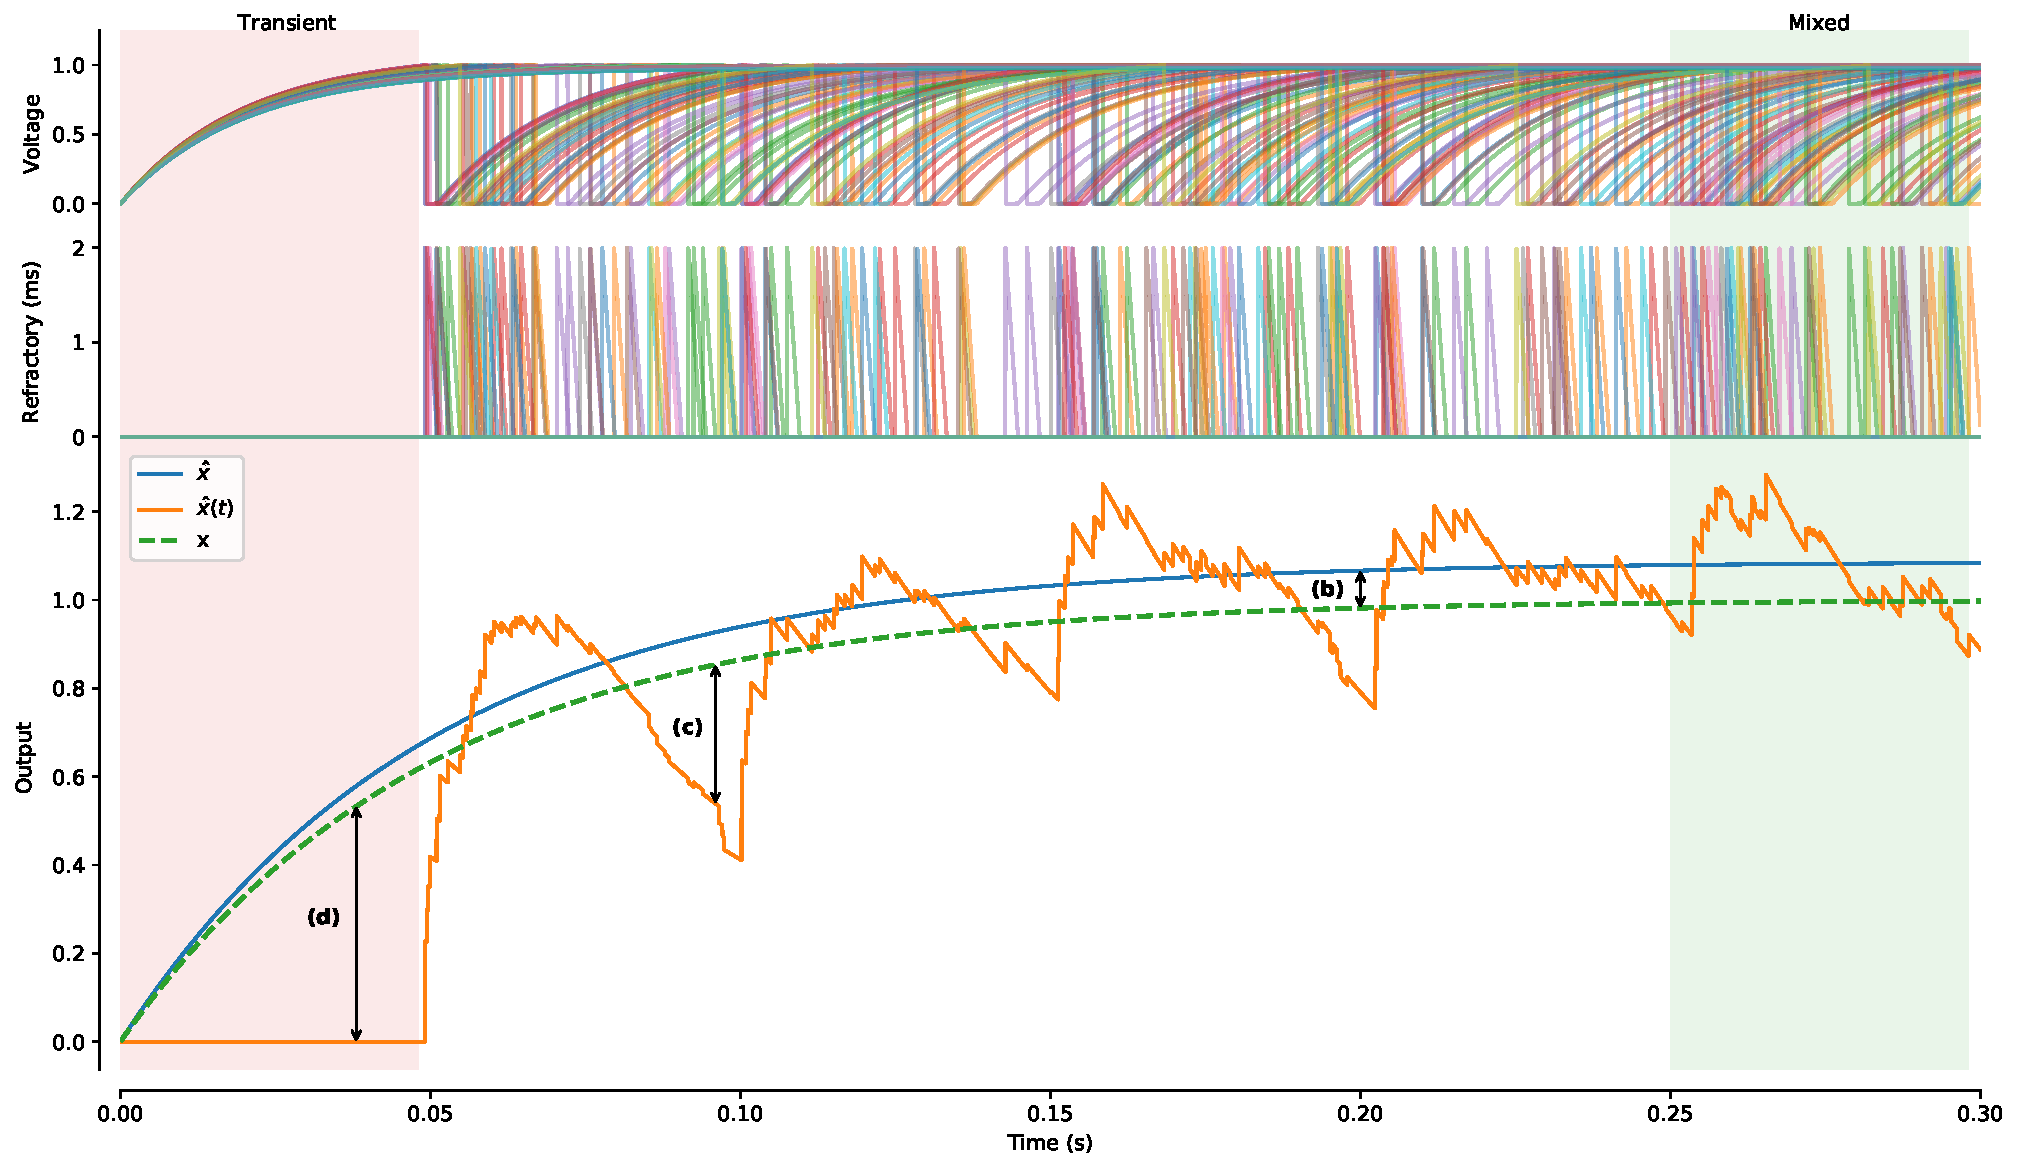
\includegraphics[width=\linewidth]{nef-error-types-a}
    \caption{Example Network Simulation}
    \label{fig:nef-error-types-a}
  \end{subfigure}
  \begin{subfigure}{.33\textwidth}
    \centering
    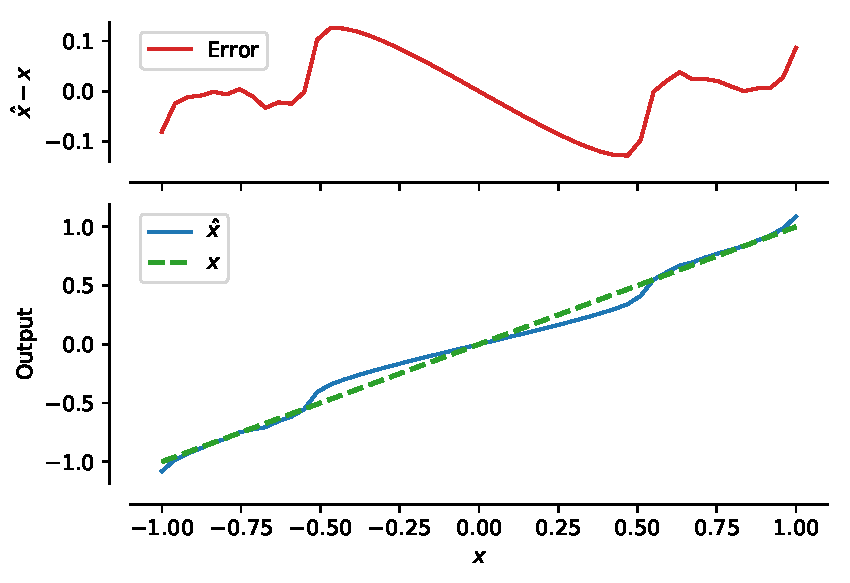
\includegraphics[width=\linewidth]{nef-error-types-b}
    \caption{Static Distortion}
    \label{fig:nef-error-types-b}
  \end{subfigure}%
  \begin{subfigure}{.33\textwidth}
    \centering
    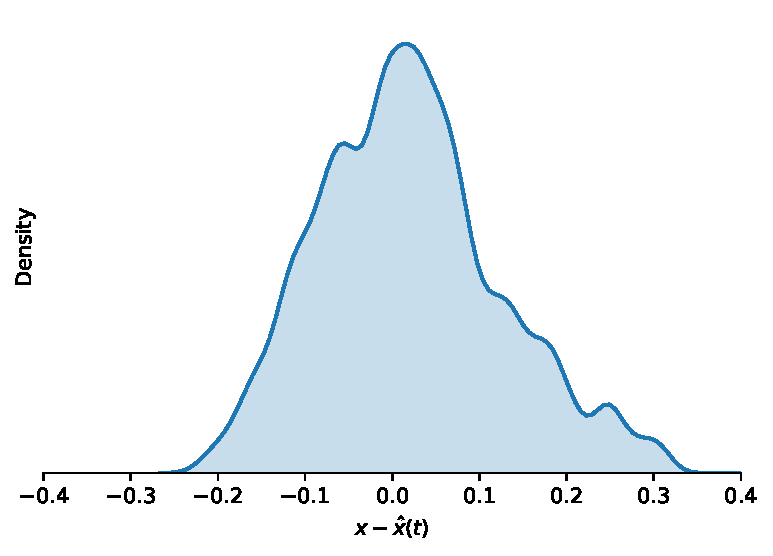
\includegraphics[width=\linewidth]{nef-error-types-c}
    \caption{Spiking Noise ($t > 0.15$\,s)}
    \label{fig:nef-error-types-c}
  \end{subfigure}%
  \begin{subfigure}{.33\textwidth}
    \centering
    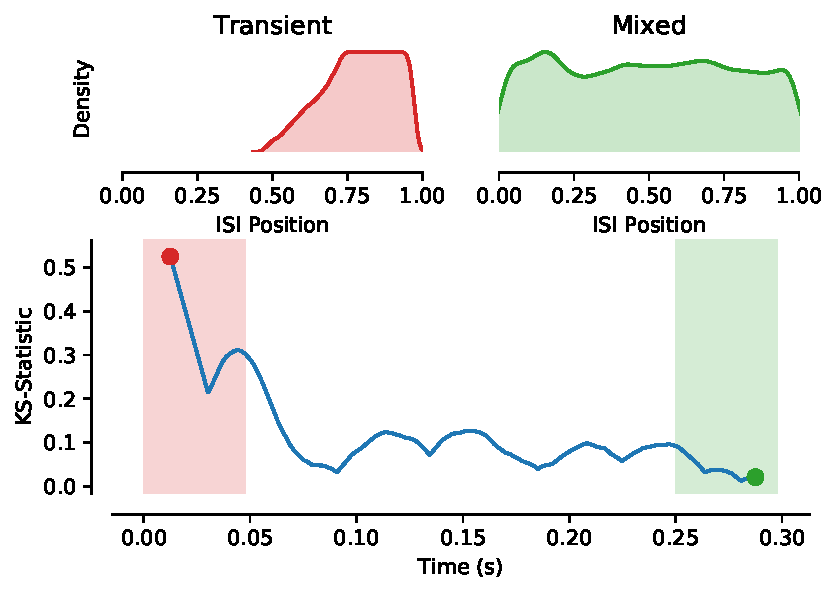
\includegraphics[width=\linewidth]{nef-error-types-d}
    \caption{State Discrepancy}
    \label{fig:nef-error-types-d}
  \end{subfigure}
  \caption{ \label{fig:nef-error-types}
    Summarizing the three types of error in a standard NEF network.
(c) Noise KS-Test: KstestResult(statistic=0.0340334175772448, pvalue=1.6183411915874764e-15)
(d) Maximum p-value: 6.984832323948373e-16
  }
\end{figure}

Mention the spike-time decoder optimization (Temporal Solver) for more detailed neurons.

Also Appendix from NEF text on synaptic versus somatic dynamics.

\subsubsection{Integrating a Spiking LIF Neuron}

We feed a constant input to a population of neurons, initially at rest, such that the the $i^{th}$ neuron spikes at a rate of $a_i$ hertz. The synapse is an integrator that will simply count spikes and output the count divided by the elapsed time $t$. This gives a one-sided estimate of the true spike rate, that is essentially equivalent to using a lowpass with infinite $\tau$.

Let $\V{\tilde{x}}(t)$ be the estimate obtained by decoding the above using the usual decoders $\V{d}$. Now observe that since $\floor{a_i t}$ is the number of times the $i^{th}$ neuron has spiked after $t$ seconds, we get:
\begin{align*}
\V{\tilde{x}}(t) &= \sum_i \V{d}_i \floor{a_i t} / t .
\end{align*}

\begin{align*}
\implies \quad \V{\hat{x}} - \V{\tilde{x}}(t) &= \sum_i \V{d}_i (a_i - \floor{a_i t} / t) \\
&= \sum_i \V{d}_i \frac{a_i t - \floor{a_i t}}{t} \\
&= \frac{1}{t} \sum_i \V{d}_i \Delta_i(t)
\end{align*}
where
\begin{align*}
\Delta_i(t) := a_i t - \floor{a_i t}, \quad 0 \le \Delta_i(t) < 1
\end{align*}
is the ``truncation'' error, obtained by rounding down to the start of the inter-spike interval at time $t$.
\begin{align*}
\implies \quad 0 \le \V{\hat{x}} - \V{\tilde{x}}(t) < \frac{1}{t} \sum_i \V{d}_i .
\end{align*}

This reveals that the error is bounded above by $O(t^{-1})$.

As an aside, since decoders grow inversely with firing rate, using neurons with higher firing rates will improve the error, as you would expect. However it is slightly counter-intuitive that adding more neurons won't increase the worst-case accuracy\footnote{The sum of all decoders is invariant to $n$.}. But observe that the worst-case is only obtained if all of the neurons collude to force $\Delta_i(t) \approx 1$ simultaneously. We will see later that less pessimistic bounds can be obtained probabilistically by assuming $\Delta_i(t)$ is sampled independently from a reasonable distribution (and then the number of neurons will matter). 

\subsubsection{Lowpass Filtering a Spiking LIF Neuron}

Suppose we feed a constant input to the $i^{th}$ neuron, which then spikes at a rate of $a_i > 0$ hertz, with the first spike occurring at some time $0 \le s_i < 1/a_i$. Filter each spike with a lowpass $h(t) = (1 / \tau) e^{-t/\tau}$. Suppose for now that the synapse is initially at rest, but this will be easy to account for at the end by linearity. % (simply add the initial state times $e^{-t/\tau}$).

Let $\tilde{a}_i(t; s_i)$ be the estimated firing rate at time $t$ given that the first spike occurs at $s_i$. By translating the above description,
\begin{align*}
\tilde{a}_i(t; s_i) &= \sum_{0 \le j \le a_i(t - s_i)} (\delta_{j / a_i + s_i} \ast h)(t) \\
&= \sum_{0 \le j \le a_i(t - s_i)} \frac{1}{\tau} e^{-(t - (j/a_i + s_i))/\tau} \\
&= \sum_{0 \le j \le a_i(t - s_i)} \frac{1}{\tau} (\underbrace{e^{-1/a_i \tau}}_{r_i})^{a_i(t - s_i) -j} 
\end{align*}
where $0 < r_i < 1$ is an important quantity that we remark is invariant to time, and depends only on the firing rate and $\tau$.
\begin{align}
\label{eq:neuron}
\implies \quad \tilde{a}_i(t; s_i) &= \frac{r_i^{a_i(t - s_i) + 1}}{\tau} \sum_{1 \le j \le a_i(t - s_i) + 1} \left( r_i^{-1} \right)^j, \quad \text{(note: change of index)} \nonumber \\
&= \frac{r_i^{a_i(t - s_i) + 1}}{\tau} \left( \frac{1}{r_i} \right) \frac{\left( \frac{1}{r_i} \right)^{\floor{a_i(t - s_i) + 1}} - 1}{\frac{1}{r_i} - 1}, \quad \text{by the geometric series} \nonumber \\
\Aboxed{ &\,= \frac{r_i^{\Delta_i(t; s_i)} - r_i^{a_i(t - s_i) + 1}}{\tau(1 - r_i)}}
\end{align}
where
\begin{equation}
\begin{gathered}
\label{eq:delta}
\Delta_i(t; s_i) := (a_i(t - s_i) + 1) - \floor{a_i(t - s_i) + 1} = a_i(t - s_i) - \floor{a_i(t - s_i)} \\
0 \le \Delta_i(t; s_i) < 1 .
\end{gathered}
\end{equation}
is again the same truncation error, but shifted to account for $s_i$. It is helpful to think of this geometrically: $\Delta_i(t; s_i)$ is simply the unit line rotated by $a_i s_i$ (modulo $1$).

\begin{figure}[h!]
\centering
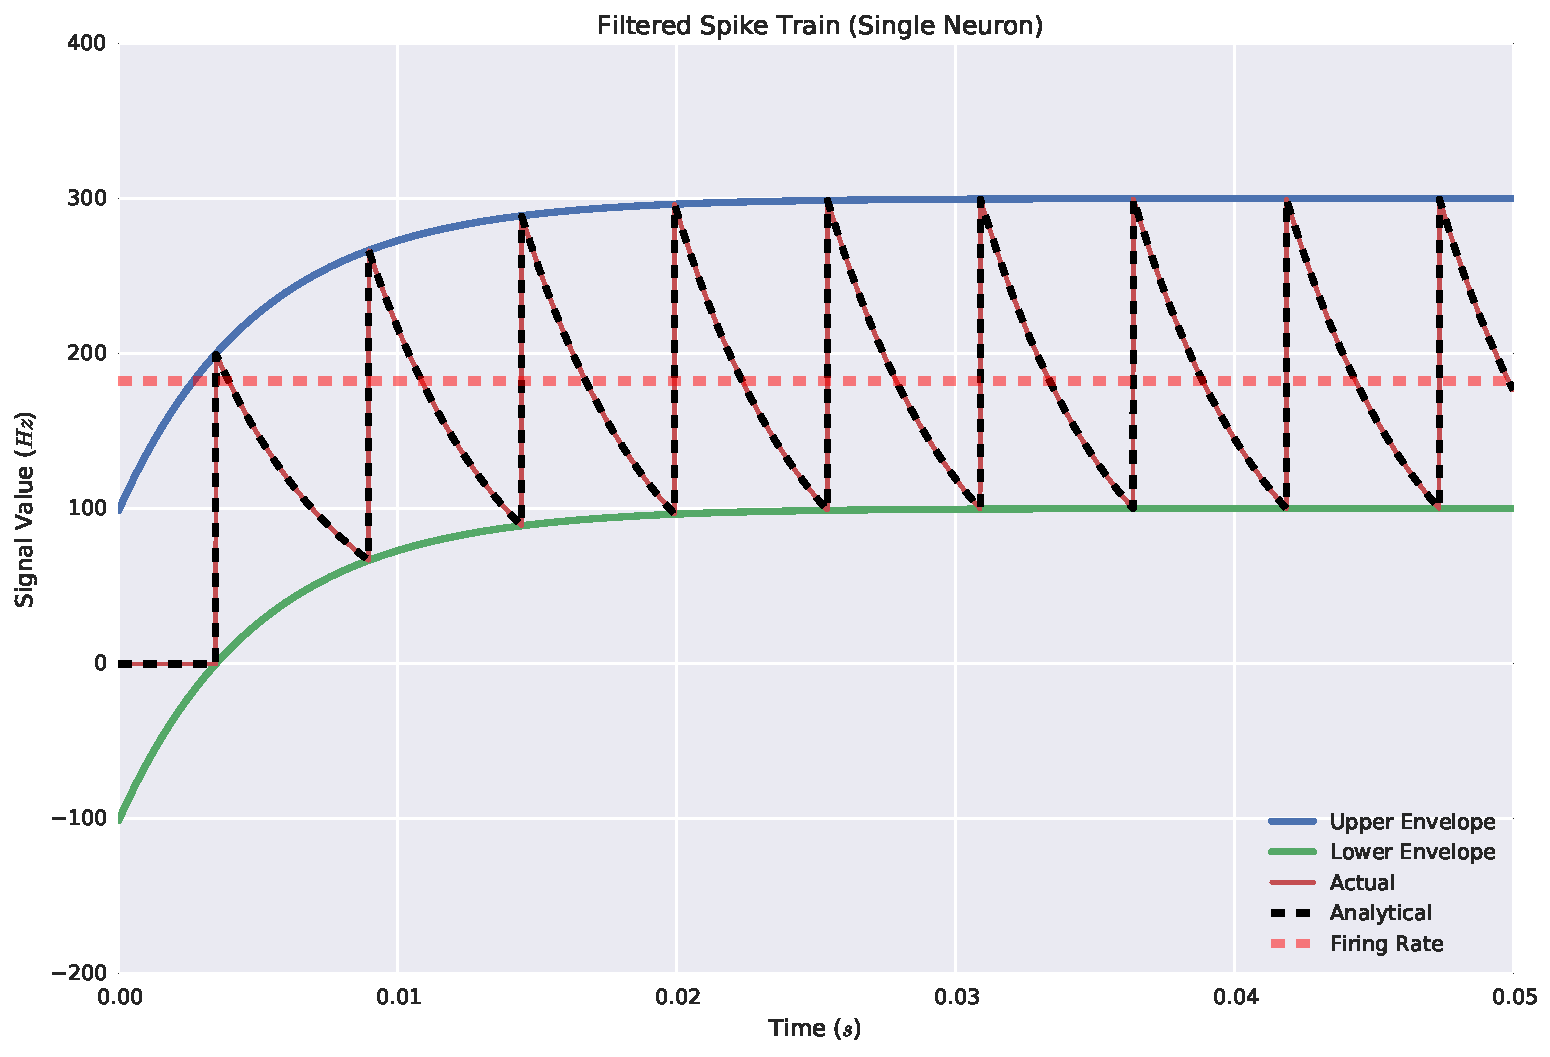
\includegraphics[width=1.0\textwidth]{slif-filtered}
\caption{\label{fig:slif-filtered} Filtered spike train under constant input ($\tau = 5\,$ms), matched by equation (\ref{eq:neuron}) and its bounds.}
\end{figure}

The boxed equation (\ref{eq:neuron}) perfectly characterizes the neuron's filtered spike train under the given assumptions. In addition, the lower/upper bounds of $\Delta_i(t; s_i)$ give the upper- and lower-envelopes, respectively:
\begin{equation*}
\frac{r_i - r_i^{a_i(t - s_i) + 1}}{\tau(1 - r_i)} < \tilde{a}_i(t; s_i) \le \frac{1 - r_i^{a_i(t - s_i) + 1}}{\tau(1 - r_i)} .
\end{equation*}

We also remark that for the LIF case, $s_i$ can be easily determined from the neuron's initial state and its input current $J_i$:
\begin{align*}
v_i(t) &= v_i(0) + (J_i - v_i(0))(1 - e^{-t/\tau_{RC}}) \\
\implies \quad s_i &= -\tau_{RC} \ln \frac{J_i - 1}{J_i}
\end{align*}
where $\tau_{RC}$ is the neuron's membrane time-constant. See \href{https://github.com/nengo/nengo/pull/975}{PR \#975} for details.

The analysis from \S\ref{sec:lowpass} can be used to obtain the precise form of the decoded estimate $\V{\tilde{x}}(t)$ at the population level. However, this depends on the initial spikes $s_i$, and so $\V{\tilde{x}}(t)$ can vary wildly depending on the initial state of all neurons.

For instance, if all neurons are initially at rest, then the estimate is most certainly zero until the fastest neuron fires. More critically, if all neurons have the same firing rate, but their initial spikes are not evenly distributed, then the error at the population level will be the addition of all their envelopes (as in the aside from the end of \S\ref{sec:integrator}).

For this work, we essentially assume that we have no control over the initial state of the system. That is, we suppose that the state of each neuron at $t = 0$ is independent and ``random'' (i.e., the previous input could have switched at any time). To be precise, we interpret $s_i$ as the realization of a random variable $S_i$ distributed by some chosen probability distribution.

Although the following analysis lends itself to the use of arbitrary distributions, some preliminary experimentation has shown that it is reasonable to assume:
\begin{equation}
\begin{gathered}
\label{eq:s}
S_i \sim U[0, 1/a_i] \\
\implies \quad f_{S_i}(s_i) = a_i \quad .  \quad \quad 
\end{gathered}
\end{equation}

This implies that the neuron is not initially biased to spike at any time in particular. In order for this to occur, we essentially require that the majority of neurons had non-zero activity in response to their prior input. In that situation, an arbitrary neuron could be at any point along its inter-spike interval, since it is not colluding with any other neurons.

In the NEF, this is typically a fair assumption, given that the tuning curves are broad (non-zero for half of the input space on average), and spike trains tend to be independent. However, for sparser encodings, or relatively large changes in input, the distribution becomes skewed towards $1 / a_i$. Similarly, if firing tends to be nearly synchronous, then the neurons will over-estimate whenever they spike together. This is noteworthy because this theory may give quantitative predictions regarding these trade-offs between encoding sparsity and firing rates, versus the desired accuracy and latency (see discussion).

Now, the analysis proceeds as follows. Fix $t$\footnote{This can be interpreted as the time that we decide to observe/measure the state of the system.} and then independently sample each $s_i$. This determines $\Delta_i(t; s_i)$ for each neuron, by the cyclic rotation $a_i s_i$ (modulo $1$) from (\ref{eq:delta}). We then define the random variable $\tilde{A}_i(t) := \tilde{a}_i(t; S_i)$, which we should understand as being distributed by ``mapping'' $S_i$ through the function $\tilde{a}_i$ for some chosen $t$. As an aside, for the special case of uniform $S_i$, the mapping $\tilde{a}_i$ actually corresponds to a cyclically shifted version of the inverse CDF of $\tilde{A}_i(t)$\footnote{This requires a subtle monotonicity argument. The CDF of $\tilde{A}_i$ can therefore be derived by inverting the unshifted $\tilde{a}_i$, but the result is not very nice to work with due to some discontinuities in its derivative.}.
%\begin{align}
%\label{eq:z}
%z_i(s_i; t) := \tilde{a}_i(t; s_i)
%\end{align}
%to view $Z_i(t)$ as a random variable that is obtained by ``mapping'' the distribution of $S_i$ through the function $\tilde{a}_i$ for some chosen $t$.  

Then the random variable $\V{\tilde{X}}(t) := \sum_i \V{d}_i \tilde{A}_i(t)$ is the decoded estimate obtained by forming a mixture of $\tilde{A}_i(t)$. The following subsections will analyze the expectation and variance of each $\tilde{A}_i(t)$ to determine the expected error and variability at time $t$.

\subsubsection{Expected Error}

By the law of the unconscious statistician (LOTUS) applied to $\tilde{A}_i(t)$:
\begin{align}
\label{eq:a_expectation}
E \left[ \tilde{A}_i(t) \right] &= \int_D \tilde{a}_i(t; s_i) f_{S_i}(s_i) \,ds_i, \quad \text{where $D$ is the domain of $S_i$} \nonumber\\
          &= \int_D \frac{r_i^{\Delta_i(t; s_i)} - r_i^{a_i(t - s_i) + 1}}{\tau(1 - r_i)} f_{S_i}(s_i) \,ds_i, \quad \text{by (\ref{eq:neuron})} \nonumber\\
          &= \frac{1}{\tau(1 - r_i)} \left( \int_0^{1} r_i^{\Delta_i(t; s_i)} \,d\Delta_i(t; s_i) - \int_0^{1/a_i} r_i^{a_i(t - s_i) + 1} (a_i) \,ds_i \right) \nonumber\\
          &= \frac{1}{\tau(1 - r_i)} \left( (-a_i \tau) e^{-\Delta_i(t; s_i)/a_i \tau} \bigg|_{\Delta_i(t; s_i) = 0}^{1} - (a_i \tau) r_i^{a_i(t - s_i) + 1} \bigg|_{s_i = 0}^{1/a_i} \right) \nonumber\\
          &= \frac{a_i}{(1 - r_i)} \left(  (1 - r_i) - (r_i^{a_i t} - r_i^{a_i t + 1})  \right) \nonumber\\
          &= a_i (1 - e^{-t/\tau}) .
\end{align}

Including the initial state of the synapse, $\V{x}_0$, the expected error at time $t$ is:
\begin{align}
\label{eq:expectation}
\implies \quad E\left[ \V{\hat{x}} - (\V{\tilde{X}}(t) + \V{x}_0 \, e^{-t/\tau}) \right] &= \sum_i \V{d}_i (a_i - E \left[ \tilde{A}_i(t) \right]) - \V{x}_0 \, e^{-t/\tau} \nonumber \\
&= \sum_i \V{d}_i a_i e^{-t/\tau} - \V{x}_0 \, e^{-t/\tau} \nonumber  \\
\Aboxed{ &\,= (\V{\hat{x}} - \V{x}_0) e^{-t/\tau} . }
\end{align}

\begin{figure}[h!]
\centering
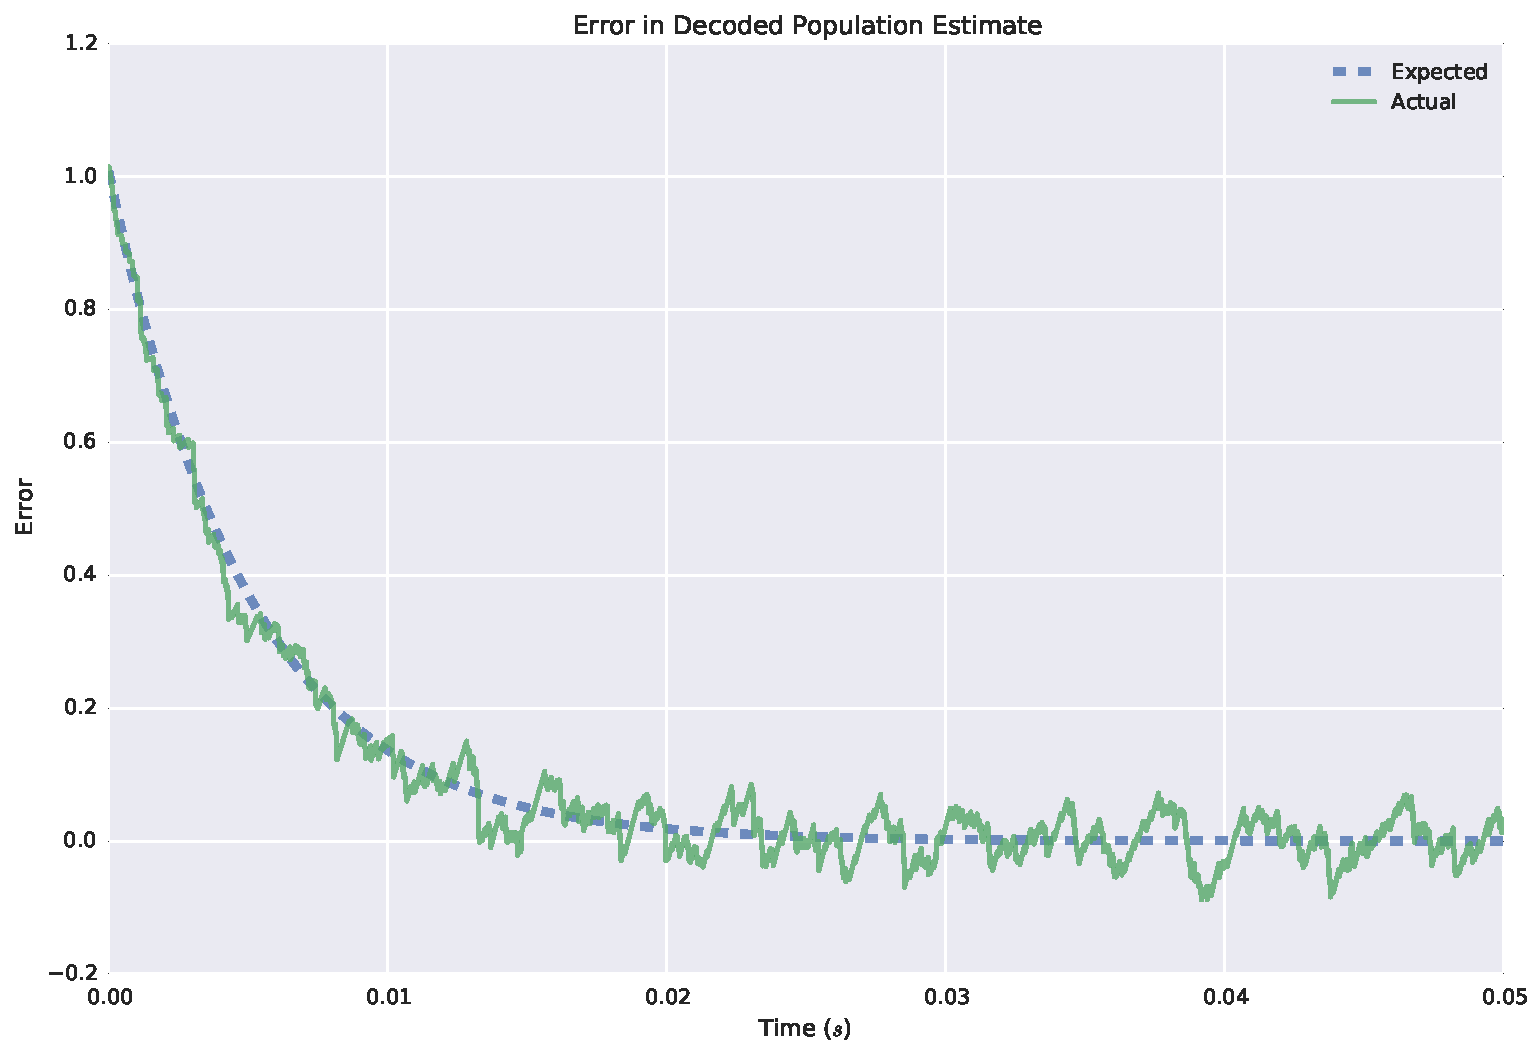
\includegraphics[width=1.0\textwidth]{slif-error}
\caption{\label{fig:slif-error} Error from filtered and decoded estimate using a population of $100$ neurons ($\tau = 5$\,ms, $\V{x}_0 = -0.2$, and $\V{\hat{x}} \approx \V{x}_0 + 1$). The expectation from (\ref{eq:expectation}) is given by the dashed line.}
\end{figure}

On one hand this is what we should intuitively expect, since we are essentially filtering an error signal using the same lowpass with an initial state given by the initial error. But it should also be surprising that this result holds independently of the width ($1 / a_i$) of each inter-spike interval, while we have only assumed the initial spikes are uniformly distributed across these intervals (in fact the independence assumption has not been used). If all neurons were initially at rest, then this result clearly no longer holds (consider $0 < t < \min_i 1/a_i$).

This assures us that we can set $\tau \rightarrow 0$ to minimize latency without hurting the expected error. However, as we will soon see, this comes at the cost of increasing the variability of the estimate.

\subsubsection{Variance in Error}

To compute $Var \left[ \tilde{A}_i(t) \right] = E \left[ \tilde{A}_i(t)^2 \right] - E \left[ \tilde{A}_i(t) \right]^2$ we rewrite the second moment:
\begin{align*}
E \left[ \tilde{A}_i(t)^2 \right] &= E \left[ \left( \frac{r_i^{\Delta_i(t; S_i)} - r_i^{a_i(t - S_i) + 1}}{\tau(1 - r_i)} \right)^2 \right] \\
&= \left( \frac{1}{\tau(1 - r_i)} \right)^2 \left( E \left[ (r_i^{\Delta_i(t; S_i)})^2 \right ] - 2 E \left[ r_i^{\Delta_i(t; S_i) + a_i(t - S_i) + 1} \right] + E \left[ (r_i^{a_i(t - S_i) + 1})^2 \right] \right)
\end{align*}
and then separately determine each expectation.

The PDFs of $r_i^{\Delta_i(t; S_i)}$ and $r_i^{a_i(t - S_i) + 1}$ are both $a_i \tau / x$ over their respective domains. This can be seen directly:
\begin{align*}
\frac{\partial}{\partial x} Pr \left[ r_i^{\Delta_i(t; S_i)} \le x \right] &= \frac{\partial}{\partial x} Pr \left[ \Delta_i(t; S_i) \le -a_i \tau \ln x \right] \\
&= \frac{\partial}{\partial x} (1 - (-a_i \tau \ln x)) \\
&= a_i \tau / x .
\end{align*}
and the proof for $r_i^{a_i(t - S_i) + 1}$ is analogous. We remark that these two facts can be used to give a slightly different derivation for (\ref{eq:a_expectation}). 

Applying LOTUS to each of these random variables gives:
\begin{align*}
E \left[ (r_i^{\Delta_i(t; S_i)})^2 \right ] &= \int_{r_i}^1 \frac{a_i \tau}{x} x^2 \,dx = \frac{a_i \tau x^2}{2} \bigg|_{x = r_i}^1 = \frac{a_i \tau (1 - r_i^2)}{2} \\
E \left[ (r_i^{a_i(t - S_i) + 1})^2 \right] &= \int_{r_i^{a_i t + 1}}^{r_i^{a_i t}} \frac{a_i \tau}{x} x^2 \,dx = \frac{a_i \tau x^2}{2} \bigg|_{x = r_i^{a_i t + 1}}^{r_i^{a_i t}} = \frac{a_i \tau (1 - r_i^2) r_i^{2 a_i t}}{2} .
\end{align*}

To compute the remaining expectation, we need to get some further understanding of $\Delta_i(t; S_i) = (a_i(t - s_i) + 1) - \floor{a_i(t - s_i) + 1}$. Define $K_i(t) := \floor{a_i t}$ as the current interval independent of $s_i$. %Then the $i^{th}$ neuron has spiked $K_i(t - s_i) + 1 = \floor{a_i(t - s_i) + 1}$ times at time $t$. More importantly, 
The point \mbox{$s_i = t - K_i(t)/a_i \equiv t \ (\text{mod}\ 1/a_i)$} gives the discontinuity in $\Delta_i(t; s_i)$ with respect to $s_i$, because that is when the spike becomes aligned with $t$ in the current interval. Namely, if $0 \le s_i \le t - K_i(t)/a_i$, then $\floor{a_i(t - s_i) + 1} = \floor{K_i(t) + 1} = K_i(t) + 1$. Likewise, if $t - K_i(t)/a_i < s_i \le 1/a_i$, then $\floor{a_i(t - s_i) + 1} = K_i(t)$\footnote{If this is confusing, recall that we are fixing $t$ and then sweeping $s_i$ from $0$ to $1 / a_i$.}. Then use LOTUS once more, along with the above fact to split up the integral.
\begin{align*}
E \left[ r_i^{\Delta_i(t; S_i) + a_i(t - S_i) + 1} \right] &= \int_0^{1/a_i} r_i^{2(a_i(t - s_i) + 1) - \floor{a_i(t - s_i) + 1}} (a_i) \, ds_i \\
&= a_i \left( \int_0^{t - K_i(t)/a_i} r_i ^ {(2a_i t - K_i(t) + 1) - (2a_i s_i)} \, ds_i + \int_{t - K_i(t)/a_i}^{1/a_i} r_i^{(2a_i t - K_i(t) + 2) - (2a_i s_i)} \, ds_i \right) \\
&= a_i r_i^{2a_i t - K_i(t) + 1} \tau / 2 \left( e^{2s_i / \tau} \bigg|_{s_i=0}^{t - K_i(t)/a_i} + r_i e^{2s_i / \tau} \bigg|_{s_i=t - K_i(t)/a_i}^{1/a_i} \right) \\
&= a_i r_i^{2a_i t - K_i(t) + 1} \tau / 2 \left( r_i^{-2 a_i(t - K_i(t)/a_i)} - 1 + r_i^{-1} - r_i^{-2a_i(t - K_i(t)/a_i) + 1} \right) \\
&= a_i \tau (1 - r_i)(r^{K_i(t) + 1} + r_i^{2a_i t - K_i(t)}) / 2
\end{align*}

Plugging these all in then gives:
\begin{align*}
Var \left[ \tilde{A}_i(t) \right] = \, \Aboxed{ a_i \left( \frac{(1 - r_i^2)(1 + r_i^{2a_i t})}{2\tau(1 - r_i)^2} - \frac{\left( r_i^{K_i(t) + 1} + r_i^{2a_i t - K_i(t)} \right)}{\tau(1 - r_i)} - a_i(1 - r_i^{a_i t})^2 \right) }
\end{align*}

\begin{align}
\label{eq:variance}
\implies \quad Var\left[ \V{\hat{x}} - (\V{\tilde{X}}(t) + \V{x}_0 \, e^{-t/\tau}) \right] = Var\left[ \V{\tilde{X}}(t) \right]
= \sum_i \V{d}_i^2 \, Var\left[ \tilde{A}_i(t) \right] .
\end{align}

\begin{figure}[h!]
\centering
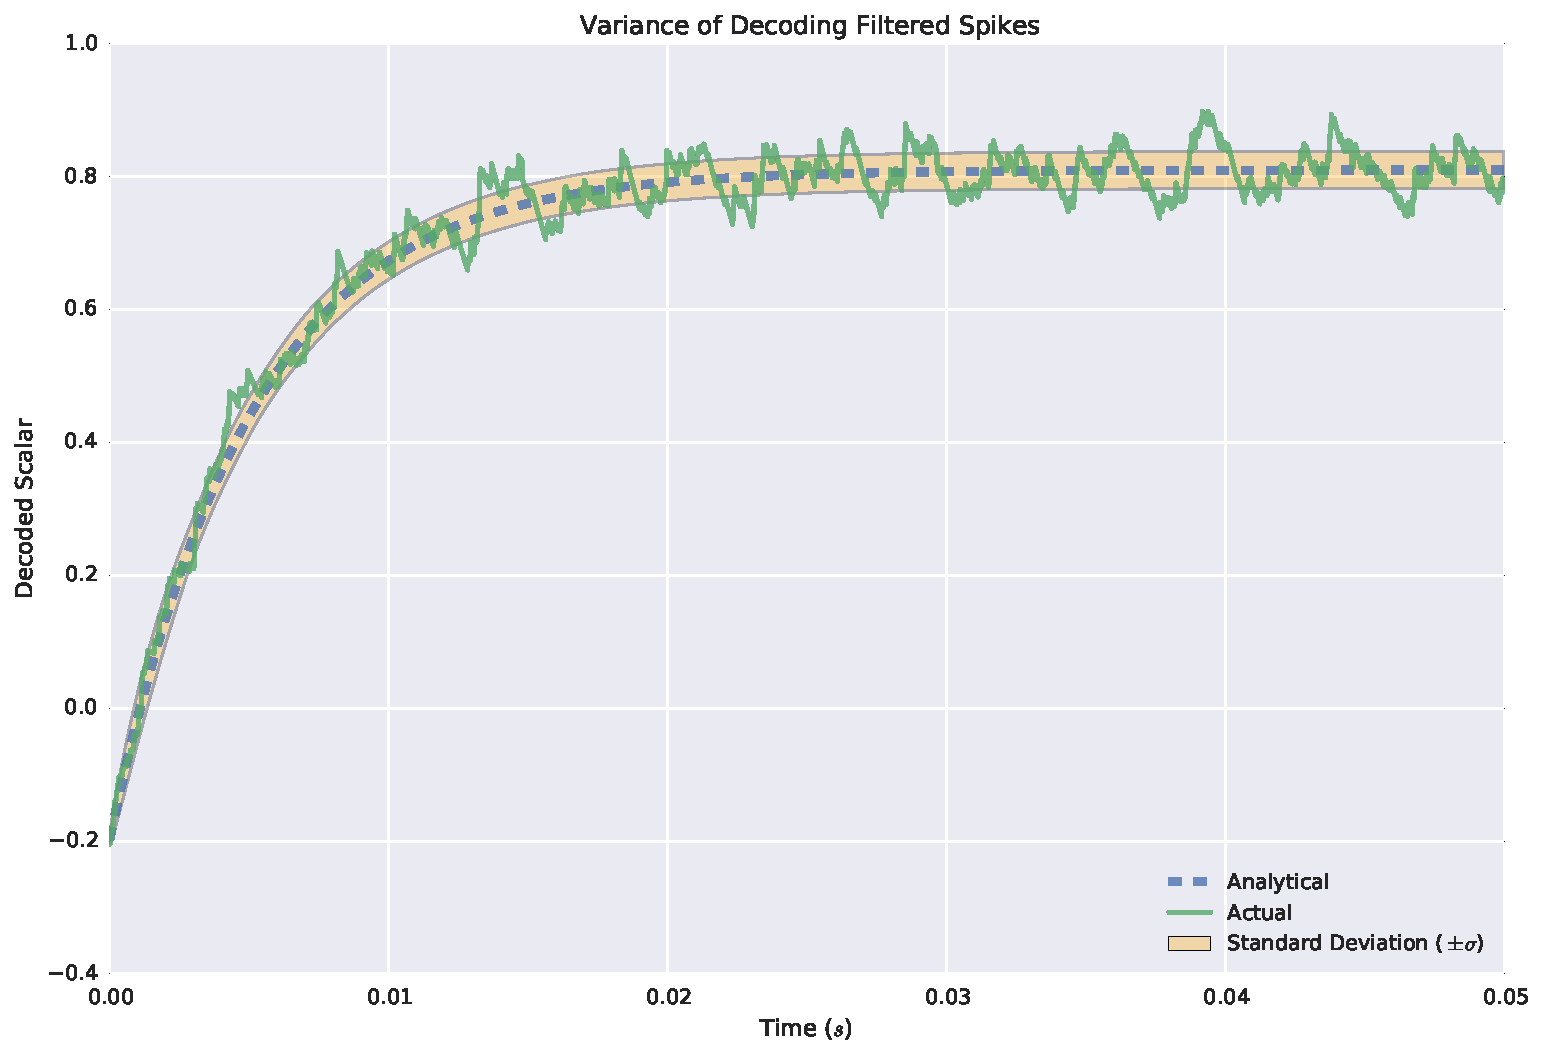
\includegraphics[width=1.0\textwidth]{slif-variance}
\caption{\label{fig:slif-variance} Filtered and decoded estimate using the same network as Fig.~\ref{fig:slif-error}. The variance is highlighted by one standard deviation from the mean.}
\end{figure}

\subsubsection{Validity of Uniform Assumption}

\begin{figure}[h!]
\centering
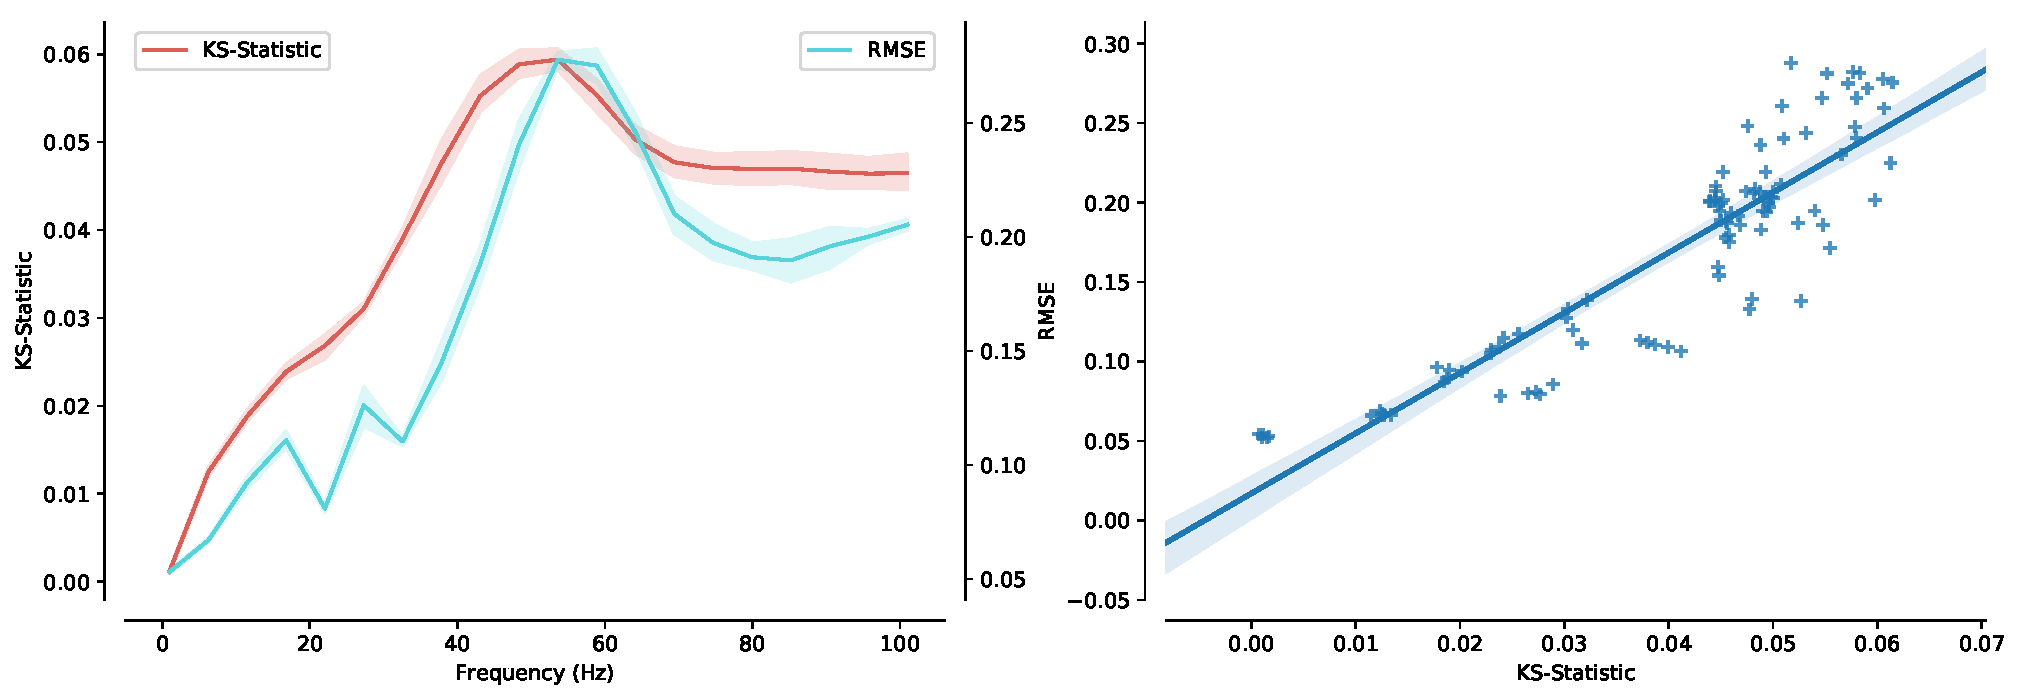
\includegraphics[width=1.0\textwidth]{frequency-ks-test}
\caption{\label{fig:frequency-ks-test}
  Relationship between the uniformity of neural states (KS-Statistic) and the representational error (RMSE) for sinusoidal stimuli of varying frequencies.
  (Left)~Empirical distribution of ISI positions---$s_i$ normalized by the instaneous rate $a_i$---is compared to the ideal uniform distribution using the Kolmogorov-Smirnov (KS) test ($p$-value~$< 0.0001$).
  % In the ideal case, the spiking LIF model is equal to its non-spiking counterpart in the sense of expectation.
  (Right)~The RMSE is highly correlated with the KS-Statistic, with a Pearson correlation coefficient of $R = 0.83$ ($p$-value~$< 0.0001$).
}
\end{figure}

The previous analysis relies on the assumption that each neuron is ``uniformly ready to spike''.
To validate this assumption from equation (\ref{eq:s}) that $S_i \sim U[0, 1/a_i]$, we empirically sampled this distribution for sinusoidal test stimuli of varying frequencies (Fig.~\ref{fig:frequency-ks-test}).
We define the \emph{ISI position} as $s_i \times a_i$. This is the realization of a random variable, in the range $[0, 1]$.
Intuitively, this can be interpreted as the percent time remaining within the idealized inter-spike interval, given the current voltage of the neuron and its ideal spike rate.
A value of $0$ implies the neuron is currently spiking and $1$ implies the neuron just spiked.
This quantity is calculated by solving the LIF ODE and rearranging to obtain:
\begin{equation}
\left(\tau_\text{RC} \log\left(1 + \frac{1 - v_i}{J_i - 1}\right) + r_i \right) a_i \text{,}
\end{equation}
where $0 \le r_i \le \tau_\text{ref}$ is the time remaining in the refractory period.

As shown in Fig.~\ref{fig:frequency-ks-test}, the default LIF model ($\tau_\text{RC} = 20$\,ms, $\tau_\text{ref} = 2$\,ms, and tuning curves uniformly distributed to achieve maximum firing rates of $50-100$\,Hz) closely follows the ideal uniform distribution ($< 6$\% error) for input frequencies up to $100$\,Hz. For $0$\,Hz (constant) inputs, the two distributions are the same (Kolmogorov-Smirnov statistic\footnote{
The maximum absolute distance between the empirical and model CDFs.
If samples are drawn from the model distribution, its Kolmogorov-Smirnov statistic approaches $0$ with probability $1$ as the number of samples approaches infinity.}%
$<0.0002$, $p$-value~$> 1-\numprint{e-15}$).
This verifies the numerics of our spiking LIF implementation\TODO{cite Nengo LIF improvements}, as we should expect that a constant input causes each neuron to spend an equal amount of time at each position within its ideal ISI.

Taken together, this means that any approximation error arising from the substitution of spiking LIF for non-spiking LIF models must arise from two sources: (1) the variability in equation \ref{eq:variance}, which is a function of $\tau$, the number of neurons, and the magnitude of the decoders, and (2) a systematic bias (Fig.~\ref{fig:frequency-ks-test}) resulting from the ISI positions being non-uniform with respect to the input stimuli.
In summary, this provides a theoretical framework for understanding the differences between spiking and non-spiking neuron models in the context of some desired PSC.
This also provides some theoretical justification for using spiking LIF models following an offline optimization using static tuning curves -- a procedure that the NEF and Nengo use regularly.
Lastly, this suggests criteria for optimizing the information-processing capabilities of spiking neurons in the context of high-frequency signals, as done in section~\ref{sec:poisson-spiking}.

\TODO{Comment on dimensional analysis for speeding up / slowing down timescales}

\subsection{Efficiency in Time and Space}

Low-rank factorization is optimal in space and time assuming linear weights (there is no advantage to factoring it any further by linearity).

\subsection{Turing-Completeness}
\label{sec:nef-turing}

A Turing machine, and a digital computer for that matter, are describable as discrete dynamical systems.
``Computing with a Distributed Reaction-Diffusion Model''


\subsection{Robustness}
\label{sec:nef-robustness}

Robustness to noise.

Also Conjecture: Den\`eve doesn't work in chaotic settings. NEF does (voltage vector is chaotic). NEF and FORCE are doing the same thing -- the latter just adds extra chaos in because Reservoir Computing.



Expose the general ideas about mapping NEF networks onto neuromorphic hardware, and what makes it better than other frameworks.


\subsection{Extensibility}
\label{sec:nef-extensibility}

Section~\ref{chapt:nef-extensions}. Loihi delay harnessing.
